\documentclass[12pt]{article}
\usepackage[utf8]{inputenc}
\usepackage[finnish]{babel}
\usepackage{graphicx}
\usepackage{float}
\usepackage{hyperref}
\title{Aineopintojen harjoitustyö: Tietokantasovellus\\Dokumentaatio}
\author{Sandra Luhtaniemi}
\begin{document}
\maketitle
\section{Johdanto}
Harjoitustyön aiheena on lankatietokanta. Tietokannan tarkoitus on tarjota käyttäjälleen väline, jolla pitää kirjaa omistamistaan eri käsityölangoista, näiden materiaalista, paksuudesta ja määrästä. Käyttäjä voi esimerkiksi kohdatessaan kiinnostavan neuleohjeen, hakea ohjeessa mainitun langan ominaisuuksien perusteella tietokannasta ne langat, joilla työ olisi mahdollista toteuttaa, sekä tarkistaa, onko hänellä sitä riittävä määrä. Käyttäjä voi myös muilla perusteilla etsiä tietokannasta lankoja, esimerkiksi vaikkapa kaikki sukkalangat. Käyttäjä voi lisätä tietokantaan uudet lankahankintansa, poistaa langan, tai päivittää sen määrän käytettyään jotakin lankaa. Järjestelmän tavoitteena on helpottaa käsitöiden suunnittelua ja vähentää turhia lankahankintoja.
\\ \ \\
Järjestelmä käyttää PostgreSQL-tietokantaa, se toteutetaan php-ohjelmointikielellä, ja se pyörii Tietojenkäsittelytieteen laitoksen users-palvelimella Apache-palvelimen alla. 
\\
\ \\
\textbf{Käyttötapaukset}\\ 
Käyttäjäryhmät:\\
Tietokannalla on vain yksi käyttäjäryhmä. Käyttäjän on rekisteröidyttävä päästäkseen käyttämään tietokantaa. Tämän jälkeen hän voi lisätä tietokantaan lankojaan ja tarkastella tai suorittaa hakuja omistamistaan langoista. 
\\ \ \\
Käyttäjän käyttötapaukset\\
Rekisteröityminen: Käyttäjä luo ensimmäisellä käyttökerralla itselleen käyttäjätunnuksen ja salasanan.
\\ \ \\
Langan lisääminen: Käyttäjä lisää tietokantaan uuden langan
\\ \ \\
Langan poistaminen: Käyttäjä poistaa tietokannasta langan, jonka on käyttänyt loppuun.
\\ \ \\
Langan määrän päivittäminen: Käyttäjä päivittää langan määrän käytettyään siitä osan.
\\ \ \\
Lankojen tarkastelu: Käyttäjä tarkastelee listaa omistamistaan langoista.
\\ \ \\
Haku ominaisuuden perusteella: Käyttäjä hakee tietokannasta kaikki jollakin ominaisuudella varustetut langat.
\\ \ \\
Omien tietojen muuttaminen: Käyttäjä muuttaa omia tietojaan, esimerkiksi salasanaansa tai nimeään.
\\ \ \\
\begin{figure}[H]
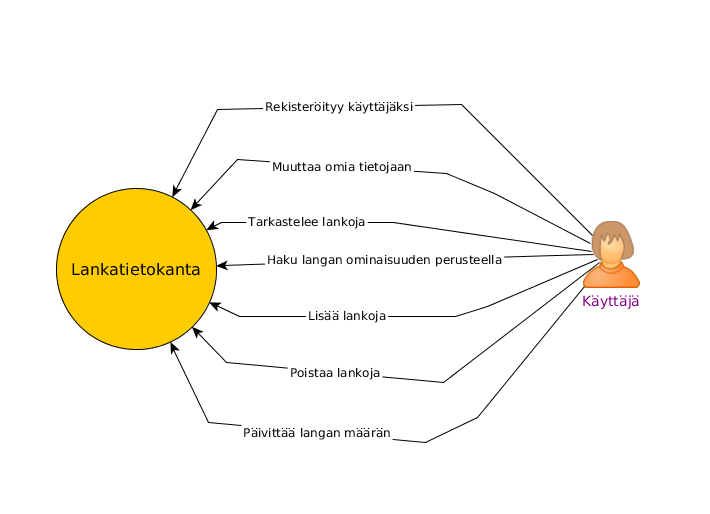
\includegraphics[scale=0.5]{sidosryhmakaavio.png}
\caption{Sidosryhmäkaavio}
\end{figure}
\begin{figure}[H]
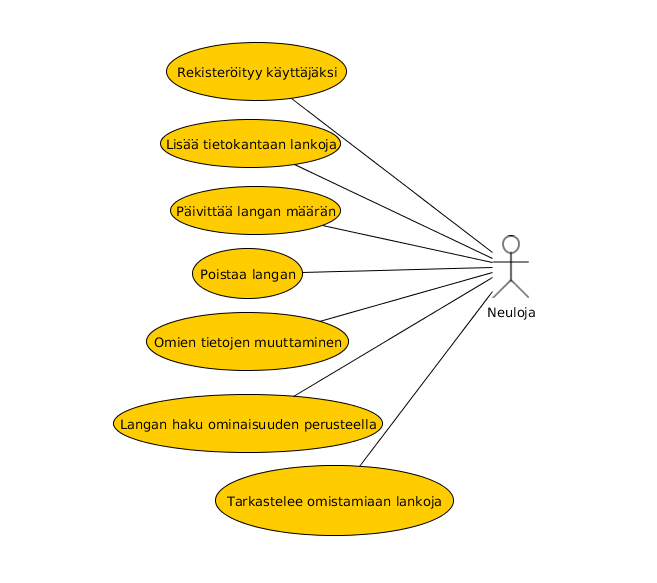
\includegraphics[scale=0.5]{kayttotapaukset.png}
\caption{Käyttötapauskaavio}
\end{figure}

\section{Käyttöliittymän suunnittelu}
Tietokohde: Yarn\\
\begin{tabular}[H]{|c|c|c|}
\hline
Attribuutti & Arvojoukko & Kuvailu \\
\hline
yarnname & Merkkijono & Langan kauppanimi \\
\hline
yarnmanu & Kokonaisluku & Langan valmistajan id-luku\\
\hline
nsrmin & Kokonaisluku & Puikkosuosituksen alaraja kerrottuna 10:llä \\
\hline
nsrmax & Kokonaisluku & puikkosuosituksen yläraja kerrottuna 10:llä \\
\hline
lpg & Kokonaisluku & Sadan gramman sisältämä metrimäärä \\
\hline  
\end{tabular}
\\
Lanka, jolla on jokin puikkosuositus, eli valmistajan antama suositus siitä minkä kokoisilla puikoilla sitä kannattaa neuloa. Puikkosuosituksella on yleensä alaraja ja yläraja, sillä käsiala voi vaihdella neulojasta riippuen. Langalle on ilmoitettu myös metrimäärä, joka sisältyy sataan grammaan, sillä sen avulla voi arvioida langan riittoisuutta.
\ \\ \ \\
Tietokohde: manu\\
\begin{tabular}{|c|c|c|}
\hline
Attribuutti & Arvojoukko & Kuvailu \\
\hline
manuname & Merkkijono & Valmistajan nimi \\
\hline
\end{tabular}
\\
Langan valmistanut yritys.
\ \\ \ \\
Tietokohde:users\\
\begin{tabular}{|c|c|c|}
\hline
Attribuutti & Arvojoukko & Kuvailu \\
\hline
username & Merkkijono & Käyttäjän valitsema käyttäjätunnus\\
\hline
password & Merkkijono & Käyttäjän valitsema salasana\\
\hline   
\end{tabular}
\\
Tietokannan käyttäjä valitsee rekisteröityessään jonkin käyttäjätunnuksen ja salasanan. 
\ \\ \ \\
Tietokohde:attr\\
\begin{tabular}{|c|c|c|}
\hline
Attribuutti & Arvojoukko & Kuvailu \\
\hline
attrname & Merkkijono & langan ominaisuus, esim. väri tai materiaali\\
\hline   
\end{tabular}
\\
Langoilla on erilaisia ominaisuuksia, esimerkiksi väri, materiaali tai vaikkapa huopuvuus tai väriin liityvä erikoisominaisuus, kuten liukuvärjäys. Langalla voi olla useita attribuutteja, ja sama attribuutti voi liittyä useaan eri lankaan. 
\ \\ \ \\
Tietokohde: owns\\
\begin{tabular}{|c|c|c|}
\hline
Attribuutti & Arvojoukko & Kuvailu \\
\hline
amount & kokonaisluku & Kayttajan omistama määrä kyseistä lankaa\\
\hline  
\end{tabular}
\\
Tietokanta voi sisältää monia eri lankoja, mutta käyttäjällä ei välttämättä ole näitä kaikkia tai eri käyttäjillä on lankoja eri määrä. 
\section{Käynnistys- ja käyttöohje}
Tietokanta löytyy osoitteesta \href{http://aluhtani.users.cs.helsinki.fi/tsoha/login.php}{http://aluhtani.users.cs.helsinki.fi/tsoha/login.php}
\\
Kirjautumista ja toimintoja voi kokeilla käyttäjätunnuksella ja salasanalla: ``Anneli'' ja "asdf''.
\section{Järjestelmän yleisrakenne}
Tietokantasovellusta tehdessä on noudatettu MVC-mallia. Kontrollerit ovat juurikansiossa. Näkymät ja malliluokat ovat kansioissa views ja lib. Apukirjastot löytyvät myös kansiosta lib. Asetukset ovat tiedostossa settings.php. Ylläpidon sivuista vastaavissa tiedostoissa on admin-etuliite. Kaikki tiedostonimet on kirjoitettu pienellä. 
\section{Järjestelmän komponentit}


\end{document}
